\documentclass{standalone}

\usepackage{tikz}
\usetikzlibrary{positioning, shapes }

\begin{document}
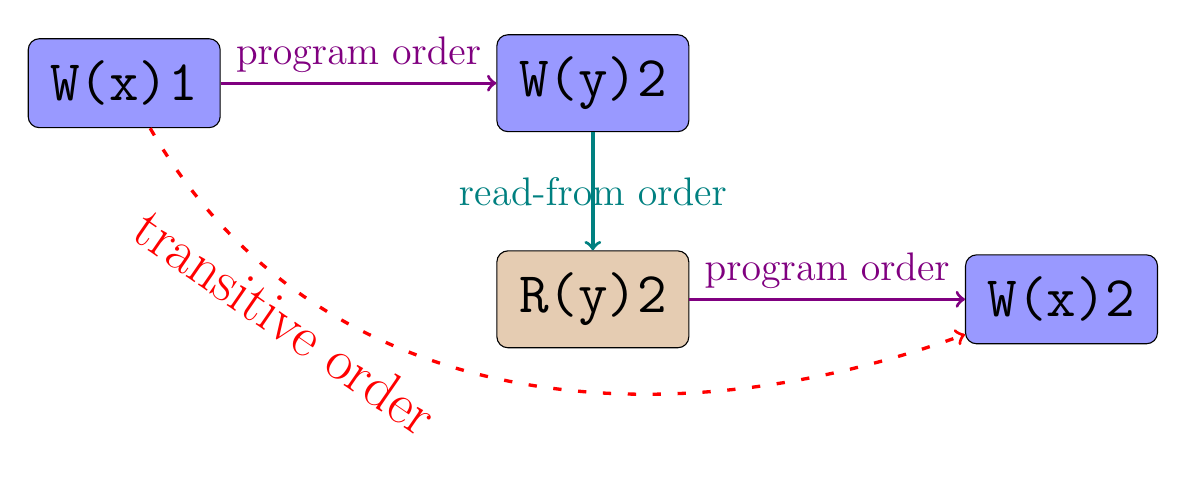
\begin{tikzpicture}
  \begin{scope}[opnode/.style = {draw, rectangle, rounded corners, fill = #1, draw, font = \huge, inner sep = 8pt}]
    \node (wx1) [opnode = blue!40] {\texttt{W(x)1}};
    \node (wy2) [opnode = blue!40, right = 3.5cm of wx1] {\texttt{W(y)2}};   
    
    \node (ry2) [opnode = brown!40, below = 1.5cm of wy2] {\texttt{R(y)2}};
    \node (wx2) [opnode = blue!40, right = 3.5cm of ry2] {\texttt{W(x)2}};       
  \end{scope}
  
  \begin{scope}
    \draw [->, very thick, violet] (wx1) to node [above, font = \Large] {program order} (wy2);
    \draw [->, very thick, teal] (wy2) to node [font = \Large] {read-from order} (ry2);    
    \draw [->, very thick, violet] (ry2) to node [above, font = \Large] {program order} (wx2);    
    \draw [->, very thick, red, loosely dashed] (wx1) to [out = -60, in = -160] node [below, font = 
    \huge, sloped, near start] {transitive order} (wx2);
  \end{scope}
\end{tikzpicture}
\end{document}
